\section{Lập trình song song trên CPU: OpenMP và MPI}

\subsection{Giới thiệu chung}
Trước khi các hệ thống gia tốc bằng phần cứng như GPU trở nên phổ biến, lập trình song song trên CPU đóng vai trò xương sống cho tính toán hiệu năng cao. Hai chuẩn thư viện phổ biến nhất đại diện cho hai mô hình bộ nhớ khác nhau là OpenMP và MPI.

\subsection{OpenMP: Mô hình bộ nhớ chia sẻ}
OpenMP (Open Multi-Processing) được thiết kế cho các hệ thống kiến trúc bộ nhớ chia sẻ (Shared Memory). Nó vận hành dựa trên cơ chế Fork-Join: chương trình bắt đầu với một luồng chính (Master Thread), sau đó phân nhánh (Fork) thành nhiều luồng con để xử lý song song các tác vụ, và gộp lại (Join) khi hoàn thành.
Để tránh xung đột dữ liệu khi dùng chung không gian bộ nhớ, OpenMP cho phép lập trình viên định nghĩa các biến chia sẻ (shared) hoặc riêng tư (private). Các biến riêng tư sẽ được cấp phát các bản sao độc lập cho mỗi luồng, đảm bảo quá trình tính toán không bị gián đoạn.

\begin{figure}[H]
    \centering
    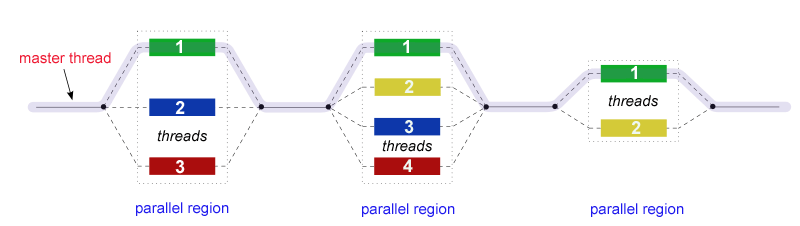
\includegraphics[width=0.6\textwidth]{Figures/OpenMP_fork_join.png}
    \caption{Cơ chế Fork-Join sinh luồng trong OpenMP}
    \label{fig:openmp_fork_join}
\end{figure}

\subsection{MPI: Mô hình truyền thông điệp}
Khác với OpenMP, MPI (Message Passing Interface) là chuẩn lập trình cho các hệ thống bộ nhớ phân tán (Distributed Memory), nơi mỗi tiến trình sở hữu một vùng nhớ độc lập. MPI sử dụng cơ chế Communicators và Rank để định danh và quản lý các tiến trình. Việc giao tiếp giữa các tiến trình được thực hiện thông qua truyền thông điệp, bao gồm giao tiếp điểm - điểm (Point-to-Point) và giao tiếp tập thể (Collective Communication).

\begin{figure}[H]
    \centering
    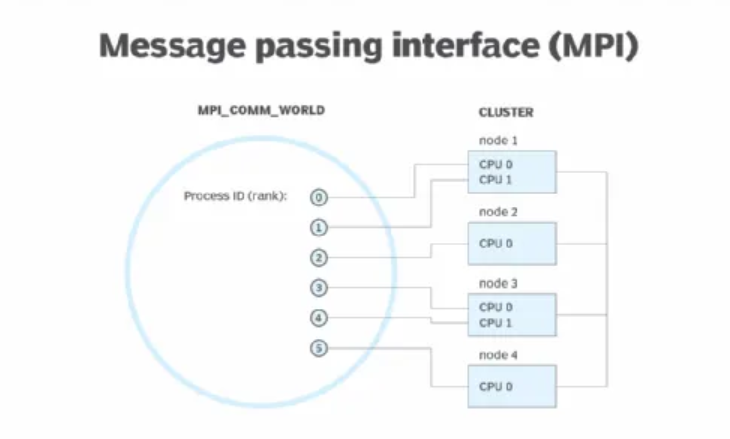
\includegraphics[width=0.6\textwidth]{Figures/MPI.png}
    \caption{Mô hình giao tiếp qua truyền thông điệp MPI}
    \label{fig:mpi}
\end{figure}

\subsection{Kết hợp OpenMP và MPI}
Trên các siêu máy tính hiện đại với kiến trúc lai (Hybrid), việc kết hợp cả hai mô hình này là rất phổ biến: OpenMP được dùng để tối ưu hóa đa luồng trên các lõi CPU bên trong cùng một node (máy chủ), trong khi MPI chịu trách nhiệm kết nối và truyền tải dữ liệu giữa các node khác nhau.

\subsection{So sánh OpenMP và MPI}
Bảng \ref{tab:openmp_mpi} tổng hợp các điểm khác biệt cốt lõi giữa hai phương pháp lập trình này.

\begin{table}[H]
\centering
\caption{So sánh đặc tính giữa OpenMP và MPI}
\label{tab:openmp_mpi}
\begin{tabularx}{\textwidth}{|X|X|}
\hline
\textbf{Đặc điểm OpenMP} & \textbf{Đặc điểm MPI} \\
\hline
Hoạt động trên mô hình bộ nhớ chia sẻ (Shared Memory). & Hoạt động trên mô hình bộ nhớ phân tán (Distributed Memory). \\
\hline
Cơ chế Fork-Join sinh luồng từ một Master Thread. & Cơ chế Communicator và Rank để quản lý các tiến trình độc lập. \\
\hline
Giao tiếp ngầm thông qua vùng nhớ chung (cần quản lý biến shared/private). & Giao tiếp tường minh thông qua truyền tin nhắn (Point-to-Point, Collective). \\
\hline
Được sử dụng chủ yếu trong nội bộ một node. & Phù hợp mở rộng quy mô tính toán giữa nhiều máy chủ (inter-node). \\
\hline
\end{tabularx}
\end{table}